\documentclass[letterpaper,11pt,twoside]{article}
../header.tex
\usepackage[margin=1in]{geometry}

\usepackage{cancel}
% email to abhinav@math.mit.edu
\def\d{\, {\rm d}}

%\usepackage{pgf,tikz}
%\usetikzlibrary{arrows}
\usepackage{wasysym}
\usepackage{pdfcomment}

\usepackage{datetime}
\usepackage{verbatim}
\usepackage[all]{xy}
\def\classnumber{18.721}
\def\classname{Algebraic Geometry}
\edef\cheadcontent{\classnumber\space Notes}

\pagestyle{fancy}
\headheight 13.7pt
\fancyhead{}
\fancyhead{Jason Gross}%\today}
\fancyfoot{}
\lhead{Jason Gross}
\rhead{\TeX ed on \today}
\chead{\cheadcontent}
\cfoot{\thepage\ of \pageref{LastPage}}

%============== Copy Diagrams ======================
\write18{mkdir "Notes by Day"}
%===================================================

\newcounter{notes-file-number}
\setcounter{notes-file-number}{0}
%mdy


%========================= Compilation ============================
\newwrite\compileout
\newtoks\filelist
\filelist={\relax}


\newcommand{\compilefilepart}[1]{%\write18{(pushd Notes by Day) & (rm "#1.pdf") & (pdflatex "#1.tex") & (rm "#1.pdf") & (pdflatex "#1.tex") & (popd)}
{\edef\temp{#1}
\global\filelist=\expandafter\expandafter\expandafter{\expandafter\temp\expandafter,\the\filelist}}%
}

\newcommand{\writeallcompiles}{
\immediate\openout\compileout compile-all.tex
\immediate\write\compileout{pushd Notes by Day}
\expandafter\writecompiles\the\filelist
\immediate\write\compileout{popd}
\immediate\closeout\compileout
\immediate\write18{mv compile-all.tex compile-all.bat}
}

\def\writecompiles#1,#2\relax{
\message{Writing compilation routine for #1^^J}
\immediate\write\compileout{(rm "#1.pdf") & (pdflatex "#1.tex") & (rm "#1.pdf") & (pdflatex "#1.tex")}
\def\second{#2}\def\emptyarg{}
\ifx#2\emptyarg
\else
  \writecompiles#2\relax
\fi}


\newcommand{\compileallfiles}{
\immediate\write18{echo Copying diagrams...} %^^J
\immediate\write18{copy /y *-*-*_Diagram_*.pdf "Notes by Day/"}
\message{Writing compilation routines...^^J}
\writeallcompiles
\immediate\write18{echo Compiling files...}%^^J}
\immediate\write18{start compile-all.bat}
}
\AtBeginDocument{\AtEndDocument{\compileallfiles}}


%================================================


\makeatletter
\newwrite\notesout

\newwrite\@notes@section@write
\newwrite\@notes@section@write@temp
\newenvironment{notessection}[3]{%
\addtocounter{notes-file-number}{1}%
\edef\notesfilenamepart{\classnumber\space Lecture Notes \twodigit{\value{notes-file-number}} - #3-\twodigit{#1}-\twodigit{#2}}%
\edef\notesfilename{"Notes by Day/\notesfilenamepart.tex"}%
\computedayofweek{#2}{#1}{#3}%
\edef\sectiontext{\dayofweeknameid{\dayofweek}, 
\ifcase#1\relax
\or January%
\or February%
\or March%
\or April%
\or May%
\or June%
\or July%
\or August%
\or September%
\or October%
\or November%
\or December%
\fi\space #2, #3}%
\immediate\openout\notesout\notesfilename
\writeheader{\notesout}%
\begingroup% Lets Keep the Changes Local
  \edef\temp{\noexpand\noexpand\noexpand\setcounter{section}{\the\value{section}}\noexpand\section{\expandafter\noexpand\sectiontext}}
  \@bsphack
  \let\@notes@section@write=\notesout
  \immediate\openout \@notes@section@write@temp \jobname.sec
  \let\do\@makeother\dospecials\catcode`\^^M\active
  \def\verbatim@processline{%
    \immediate\write\@notes@section@write{\the\verbatim@line}%
    \immediate\write\@notes@section@write@temp{\the\verbatim@line}}%
  \expandafter\verbatim@start
  \temp}%
{{\let\end=\relax\immediate\write\@notes@section@write{\end{document}}}%
 \immediate\closeout\@notes@section@write
 \immediate\closeout\@notes@section@write@temp\@esphack\endgroup%
 \compilefilepart{\notesfilenamepart}
\input{\jobname.sec}%
}%







\catcode`\^^M\active
\newcommand{\writeheader}[1]{\begingroup
\let\ =\relax
\let\,=\relax
\let\RelativitySection=\relax
\let\TeX=\relax
\let\begin=\relax
\let\cfoot=\relax
\let\chead=\relax
\let\cheadcontent=\relax
\let\d=\relax
\let\def=\relax
\let\documentclass=\relax
\let\fancyfoot=\relax
\let\fancyhead=\relax
\let\hbox=\relax
\let\headheight=\relax
\let\input=\relax
\let\kern=\relax
\let\leavevmode=\relax
\let\lhead=\relax
\let\lower=\relax
\let\newcommand=\relax
\let\oldsection=\relax
\let\pageref=\relax
\let\pagestyle=\relax
\let\raise=\relax
\let\rhead=\relax
\let\rm=\relax
\let\scriptfont=\relax
\let\section=\relax
\let\sfrac=\relax
\let\the=\relax
\let\thepage=\relax
\let\today=\relax
\let\usepackage=\relax
\let\let=\relax
\edef\temp{\documentclass[letterpaper,11pt,twoside] {article}
%\usepackage{pst-pdf,pst-text,pstricks-add}
\providecommand{\ifincludeall}{\iffalse}
\usepackage{fancyhdr}
\usepackage{lastpage}
\usepackage{enumerate}
\ifincludeall

  \usepackage{wrapfig}

%================================ Unicode ================================
  \usepackage[utf8]{inputenc}
  \DeclareUnicodeCharacter{916}{\ensuremath{\Delta}}
  \DeclareUnicodeCharacter{937}{\ensuremath{\Omega}}
  \DeclareUnicodeCharacter{949}{\ensuremath{\epsilon}}
  \DeclareUnicodeCharacter{956}{\ensuremath{\mu}}
  \DeclareUnicodeCharacter{963}{\ensuremath{\sigma}}
  \DeclareUnicodeCharacter{977}{\ensuremath{\theta}}
  \DeclareUnicodeCharacter{1009}{\ensuremath{\rho}}
  \DeclareUnicodeCharacter{03B4}{\ensuremath{\delta}}
  \DeclareUnicodeCharacter{221A}{\sqrt}
  \DeclareUnicodeCharacter{2124}{\ensuremath{\mathbb Z}}
%============================== End Unicode ==============================
\fi


\usepackage{amsmath}
\usepackage{amssymb}
%================================= AMSTHM =================================
\usepackage{amsthm}

\newtheorem{thm}{Theorem}[section]
%\newtheorem{theorem}{Theorem}
\newtheorem{conjecture}{Conjecture}[section]
\newtheorem{lem}{Lemma}[section]
%\newtheorem{lemma}[theorem]{Lemma}
\newtheorem{cor}[thm]{Corollary}
%\newtheorem{corollary}[theorem]{Corollary}
\newtheorem{prop}[thm]{Proposition}
%\newtheorem{proposition}[theorem]{Proposition}
%\newtheorem{definition}[theorem]{Definition}
%\newtheorem{example}[theorem]{Example}
\newtheorem{exercise}[thm]{Exercise}
%\newtheorem{exercise}[theorem]{Exercise}
\newtheorem{claim}[thm]{Claim}
\newtheorem{law}{Law}[section]
\newtheorem*{thm*}{Theorem}
\newtheorem*{lem*}{Lemma}
\newtheorem*{conjecture*}{Conjecture}
\newtheorem*{cor*}{Corollary}
\newtheorem*{prop*}{Proposition}
\newtheorem*{exercise*}{Exercise}
\newtheorem*{law*}{Law}
\newtheorem*{claim*}{Claim}



\theoremstyle{definition} \newtheorem{defn}{Definition}[section]
\theoremstyle{definition} \newtheorem*{defn*}{Definition}
\newtheorem{example}[thm]{Example}
\newtheorem*{example*}{Example}
\newtheorem{eg}[thm]{Example}
\newtheorem*{eg*}{Example}

\newtheorem{fact}{Fact}[section]
\newtheorem*{fact*}{Fact}

\newcommand{\thmref}[1]{Theorem~\ref{#1}}
%=============================== End AMSTHM ===============================
\usepackage{esint}
\ifincludeall
  \usepackage[table]{xcolor}
  \usepackage{xifthen}
\fi
%\if dcpic
%\usepackage{dcpic}
%\else

%\ifincludeall
  \usepackage{ifpdf}
%\else
  %\newif\ifpdf
  %\pdftrue
%\fi

\ifincludeall
  \ifpdf
    \usepackage[pdftex]{graphicx}
    \usepackage{pdfpages}
    \usepackage[plainpages=false,pdfpagelabels,unicode]{hyperref}
  \else
    \usepackage[dvips]{graphicx}
    \usepackage{pstricks,pstricks-add,pst-math,pst-xkey}
  \fi
\else
  \usepackage[pdftex]{graphicx}
  \usepackage[pdfpagelabels,unicode]{hyperref}
\fi

%\ifincludeall
  \usepackage{mathtools}
%\fi

%\global\def\isxy{}
%\global\let\isxy\relax
\ifincludeall
  \providecommand{\isxy}{\let\isxy\relax}
  \expandafter\ifx\isxy\relax
    %\usepackage{mathpazo} or \usepackage{mathptmx} 
    \usepackage{flexisym} % flexisym package is required by breqn
                          % can load as \usepackage[mathpazo]{flexisym}
    \usepackage{breqn}
  \else
    \usepackage[all]{xy}
  \fi
\fi



%\usepackage[exponent-product=\cdot,per-mode=fraction,quotient-mode=fraction,fraction-function=\sfrac]{siunitx} %alsoload={named,prefixed,abbr,hep},
%\newunit{\statvolt}{statV}
%\newunit{\erg}{erg}
%\newunit{\esu}{esu}

\providecommand{\abs}[1]{\left\lvert#1\right\rvert}%\DeclarePairedDelimiter\abs{\lvert}{\rvert} %\providecommand{\abs}[1]{\lvert#1\rvert}
\ifincludeall
  \DeclarePairedDelimiter\norm{\lVert}{\rVert}
  \DeclarePairedDelimiter\floor{\lfloor}{\rfloor}
\else
  \providecommand{\floor}[1]{\left\lfloor #1\right\rfloor}
  \providecommand{\norm}[1]{\lVert#1\rVert}
\fi
\newcommand{\gcdf}[2]{\left( #1 , #2 \right)}
\DeclareMathOperator{\lcm}{lcm}
\DeclareMathOperator{\im}{im}
\DeclareMathOperator{\rank}{rank}
\DeclareMathOperator{\spans}{span}
\DeclareMathOperator{\divergence}{div}
\DeclareMathOperator{\tr}{tr}
\DeclareMathOperator{\grad}{grad}
\DeclareMathOperator{\spec}{Spec}
\DeclareMathOperator{\pspec}{PSpec}
\DeclareMathOperator{\rad}{rad}
\DeclareMathOperator{\trdeg}{tr\,deg}
\DeclareMathOperator{\gk}{gk}
\DeclareMathOperator{\fract}{fract}
\newcommand{\lcmf}[2]{\lcm\left( #1 , #2 \right)}
\def\dbar{{\mathchar'26\mkern-12mu d}}

\def\sfrac#1/#2{\leavevmode\kern.1em\raise.5ex\hbox{\the\scriptfont0 #1}\kern-.1em/\kern-.15em\lower.25ex\hbox{\the\scriptfont0 #2}}

\renewcommand{\d}{\,d}

\newcommand{\defeq}{\coloneqq}%\stackrel{\mathrm{df}}{=}}%{\ensuremath{:=}}%

\ifincludeall
  \newcommand{\complementset}[1][\ \ \rule{0pt}{1ex}]{\overline{#1}}
  \newcommand{\boldcomplementset}[1][\ \ \rule{0pt}{1ex}]{\text{\makebox[0pt][l]{$#1$}}\rule[\heightof{#1}+3pt]{\widthof{#1}}{0.11ex}}
  \let\oldboldsymbol=\boldsymbol
  \renewcommand{\boldsymbol}[1]{\let\oldcomplementset=\complementset%
  %\oldboldsymbol{#1}\  	%
  \let\complementset\boldcomplementset%
  \oldboldsymbol{#1}%
  \let\complementset=\oldcomplementset}
\fi
% \gdef\phantomhdepth{\relax}
% \gdef\phantomhdepth{1}
% \newcommand{\phantomheight}[1]{         %
% \ifx\phantomhdepth\relax          %
%   \let\phantomhdepth{1}          %
%   \vphantom{#1}          %
%   \let\phantomhdepth\relax          %
% \fi          %
% }
\newcommand{\tuple}[1]{\breakingtuple{#1}}
\newcommand{\nbtuple}[1]{\left(#1\right)}
\newcommand{\breakingtuple}[1]{\lrbreak{(}{#1}{)}}         %$
         %\let\oldcomma=,
\begingroup
  \lccode`~=`,
  \lowercase{\endgroup
    \let\oldcomma=~
    \def\comma{\oldcomma}
    \def~{\comma}         %
  }         %
         %\def\aaa{\comma}
         %\mathcode`,="613B

\newcommand{\allowbreaks}[1]{\begingroup \mathcode`,="8000 \def\comma{\oldcomma\allowbreak}#1\def\comma{\oldcomma} \mathcode`,="613B \endgroup }         %\replace{#1}{,}{,\allowbreak}}
%\let\phantomheight\vphantom
\newcommand{\lbreakh}[4][\!\!]{\left#2\vphantom{#3#4}\right.#1\allowbreaks{#3}}
\newcommand{\rbreakh}[4][\!\!]{#2#1\left.\vphantom{#2#4}\right#3}
\newcommand{\lrbreakh}[5][\!\!]{\left#2\vphantom{#3#5}\right.#1\allowbreaks{#3}#1\left.\vphantom{#3#5}\right#4}
\newcommand{\lbreak}[3][\!\!]{\lbreakh[#1]{#2}{#3}{}}
\newcommand{\rbreak}[3][\!\!]{\rbreakh[#1]{#2}{#3}{}}
\newcommand{\lrbreak}[4][\!\!]{\lrbreakh[#1]{#2}{#3}{#4}{}}
\newcommand{\olrbreak}[5][\!\!]{\overlineb{\lrbreakh[#1]{#2}{#3}{.}{#4}}{\lrbreakh[#1]{.}{#4}{#5}{#3}}}
\newcommand{\olrbreakc}[6][\!\!]{\overlineb{#2\lbreakh[#1]{#3}{#4}{#5}}{\rbreakh[#1]{#5}{#6}{#4}}}%\lrbreak[#1]{.}{#5}{#5}}}

%\DeclarePairedDelimiter\simpleset{\lbrace}{\rbrace}
\newcommand{\simpleset}[1]{\left\lbrace#1\right\rbrace}
\newcommand{\simplesetb}[1]{\lrbreak{\lbrace}{#1}{\rbrace}}

\newcommand{\mathsetb}[2][\relax]{%
\ifx#1\relax
  \simplesetb{#2}
\else
  \simplesetb{\suchthatb[#1]{#2}}
\fi}

\newcommand{\mathset}[2][\relax]{%
\ifx#1\relax
  \simpleset{#2}
\else
  \simpleset{\suchthat[#1]{#2}}
\fi}
\newcommand{\omathset}[3][\relax]{%
\ifx#1\relax
  \overlineb{\lrbreak{\lbrace}{#2}{.}}{\lrbreak{.}{#3}{\rbrace}}
\else
  \overlineb{\lrbreak{\lbrace}{\suchthat[#1]{#2}}{.}}{\lrbreak{.}{#3}{\rbrace}}
\fi}

\newcommand{\omathsetc}[4][\relax]{%
\ifx#1\relax
  \overlineb{\lrbreak{\lbrace}{\suchthat[#2]{#3}}{.}}{\lrbreak{.}{#4}{\rbrace}}
\else
  \overlineb{#1\lrbreak{\lbrace}{\suchthat[#2]{#3}}{.}}{\lrbreak{.}{#4}{\rbrace}}
\fi}
  
\newcommand{\overlinet}[2]{\overlineb{#1}{#2}}
\newcommand{\overlineb}[2]{\overline{#1\vphantom{#2}}\allowbreak\overline{#2\vphantom{#1}}}
%\newcommand{\overlinec}[3]{\overline{#1\text{\makebox[0pt]{$\phantom{#2#3}$}}}\allowbreak\overline{#2\vphantom{#1#3}}\allowbreak\overline{#3\vphantom{#1#2}}}

\newcommand{\suchthat}[2][]{#1\left\vert\vphantom{#1#2}\right.\!#2}
\newcommand{\suchthatb}[2][]{#1 \lbreakh[\!]{\vert}{#2}{#1}}
\providecommand{\scfont}{}

%texbook
%\newif\ifv@ \newif\ifh@
%\def\vphantom{\v@true\h@false\ph@nt}
%\def\hphantom{\v@false\h@true\ph@nt}
%\def\phantom{\v@true\h@true\ph@nt}
%\def\ph@nt{\ifmmode\def\next{\mathpalette\mathph@nt}%
%\else\let\next=\makeph@nt\fi \next}
%\def\makeph@nt#1{\setbox0=\hbox{#1}\finph@nt}
%\def\mathph@nt#1#2{\setbox0=\hbox{$\m@th#1{#2}$}\finph@nt}
%\def\finph@nt{\setbox2=\null \ifv@ \ht2=\ht0 \dp2=\dp0 \fi
%\ifh@ \wd2=\wd0 \fi \box2 }


%\def\m@th{\mathsurround=0pt }
\def\uncurry#1#2{#1#2} % \uncurry\macro1{{arg1}{arg2}...} -> \macro1{arg1}{arg2}...
\def\curryone#1#2#3{{\def\ndef{\noexpand\def}\def\first{\noexpand#1}\expandafter}\ifx\ndef\first #1{#2{#3}}\else #1{{#2}{#3}}\fi}
\def\currytwo#1#2#3#4{#1{{#2}{#3}{#4}}}
\def\currythree#1#2#3#4#5{#1{{#2}{#3}{#4}{#5}}}
\def\curryfour#1#2#3#4#5#6{#1{{#2}{#3}{#4}{#5}{#6}}}
\def\curryfive#1#2#3#4#5#6#7{#1{{#2}{#3}{#4}{#5}{#6}{#7}}}
\def\currysix#1#2#3#4#5#6#7#8{#1{{#2}{#3}{#4}{#5}{#6}{#7}{#8}}}
\def\curryseven#1#2#3#4#5#6#7#8#9{#1{{#2}{#3}{#4}{#5}{#6}{#7}{#8}{#9}}}


\def\uncurrytwo#1#2#3{#1#2#3}
\def\uncurriedmathpalette#1{\def\uncurried{\uncurrytwo#1}\mathpalette\uncurried}
\def\mathpalettetwo#1#2#3{\uncurriedmathpalette{#1}{{#2}{#3}}}
\def\mathpalettethree#1#2#3#4{\uncurriedmathpalette{#1}{{#2}{#3}{#4}}}


%\def\aswidthof{\v@false\h@true\@sof}
%\def\asheightof{\v@true\h@false\@sof}
%\def\assizeof{\v@true\h@true\@sof}

%\newcommand{\@sof}[3][l]{\ifmmode \def\next{\mathpalettethree\math@sof}%
%\else\let\next=\make@sof\fi \next{#1}{#2}{#3}}
%
%\def\make@sof#1#2#3{\setbox0=\hbox{#2}\setbox2=\makebox[0pt][c]{#3}\fin@sof}
%\def\math@sof#1#2#3{\setbox0=\hbox{$\m@th#1{#2}$}\setbox2=\hbox{$\m@th#1{#3}$}\fin@sof}
%\def\fin@sof{\ifv@ \ht2=\ht0 \dp2=\dp0 \fi
%\ifh@ \wd2=\wd0 \fi \box2 }
\makeatletter
\newcommand{\aswidthof}[3][c]{\ifmmode \def\next{\mathpalettethree\m@th@swidthof}%
\else\let\next=\m@ke@swidthof\fi \next{#1}{#2}{#3}}

\newdimen\@widthof
\newcommand{\m@th@swidthof}[4]{\text{\settowidth\@widthof{$\m@th#1#3$}\makebox[\@widthof][#2]{$\m@th#1#4$}}}
\newcommand{\m@ke@swidthof}[3]{\settowidth\@widthof{#2}\makebox[\@widthof][#1]{#3}}


%
%
%
%
%
%\makeatletter
%
%\def\aswidthof{\v@false\h@true\@sof}
%\def\asheightof{\v@true\h@false\@sof}
%\def\assizeof{\v@true\h@true\@sof}
%
%\def\@sof{\ifmmode\def\next##1##2{\mathpalette{\math@sof##1##2}}%
%\else\let\next=\make@sof\fi \next}
%
%\def\make@sof#1#2{\setbox0=\hbox{#1}\setbox2=\hbox{#2}\fin@sof}
%\def\math@sof#1#2#3{\setbox0=\hbox{$\m@th#3{#1}$}\setbox2=\hbox{$\m@th#3{#2}$}\fin@sof}
%\def\fin@sof{\ifv@ \ht2=\ht0 \dp2=\dp0 \fi
%\ifh@ \wd2=\wd0 \fi \box2 }

%\text{\newdimen\tempwidth \settowidth\tempwidth{$#3$}\makebox[\tempwidth][#1]{$#2$}}}% \text{\raisebox{0ex}[-\height][-\height]{$\phantom{#2}$}}}
%\newcommand{\asheightof}[3]{#1\text{\makebox[0pt]{$\phantom{#2}$}}\right.#2\left.\text{\makebox[0pt]{$\phantom{#2}$}}#3}

% 276887 sp is twice the width difference between $\left(\right)$ and $\left(\right.\left.\right)$
% \hspace{-138444 sp} \hspace{-138443 sp}\
\makeatletter
\def\breakingleft#1{{\def\templeft##1\breakingright##2{\left#1\vphantom{##1}\right.\n@space##1\n@space\left.\vphantom{##1}\right##2}\expandafter}\templeft}

\newcommand{\fullexpand}[2][]{{#1\edef\temp{#2}\expandafter}\temp}
\def\settoksexpanded#1=#2{{\edef\temp{{#2}}\expandafter}\expandafter#1\expandafter=\temp}

\newcommand{\selectfontsize}[1]{\fontsize{#1}{#1}\selectfont}

\newcommand{\newlinep}{$\left.\right.$\par\noindent}

\makeatletter
\newcommand{\interitemtext}[1]{%
\begin{list}{}
{\itemindent=0mm\labelsep=0mm
\labelwidth=0mm\leftmargin=0mm
\addtolength{\leftmargin}{-\@totalleftmargin}}
\item #1
\end{list}}
\makeatother


\newcommand{\ncr}[2]{\binom{#1}{#2}}
\newcommand{\definition}[1]{\begin{defn}#1\end{defn}}%{\par \noindent {\bf Definition:} #1}
\newcommand{\factc}[1]{\par \noindent \underline{\bf Fact:} #1}
%\providecommand{\lrang}[1]{\left\langle#1\right\rangle}%\DeclarePairedDelimiter\lrang{\langle}{\rangle}
\providecommand{\WLOG}{Without loss of generality}
\providecommand{\TFAE}{The following are equivalent}%{These facts are excellent}%(Ari)
\def\<#1>{\left\langle#1\right\rangle}
\def\[#1]{\left[#1\right]}
%\def\{#1|#2}{\mathset[#1]{#2}}
\providecommand{\End}[1]{\mathop{End}\left(#1\right)}
\providecommand{\dom}[1][\relax]{\mathop{dom}%
\ifx#1\relax%
\else%
  \left(#1\right)%
\fi}

\providecommand{\ses}{short exact sequence}
\providecommand{\st}{such that}


\newenvironment{digression}{\noindent\begin{math}%
\left(\ \begin{minipage}{0.95\textwidth}% FIX: Make this more robust
  }{\end{minipage}\ \right)\end{math}}

%\newenvironment{correction}{\textcolor{red}}{}
%======================================== Physics ===================================================
\providecommand{\uvec}[1]{{\widehat{\bf{#1}}}}
%\MakeAtOther
%\providecommand{\declareunits}[1][km,m,cm,mm,s,L,mL,kg,g]{%
%\@for\@unit:=#1\do{%
%  \declareunit{\@unit}%
%}}
%\providecommand{\declareunit}[2][\relax]{\ifx#1\relax%
%  \def\csname #2\endcsname{\text{#2}}%
%\else
%  \def\csname #1\endcsname{\text{#2}}%
%\fi}
%====================================================================================================

%================================= Proof Cases ===============================
\newcounter{ProofCasesLvlCtr}
\newcounter{ProofCasesMaxCtr}
\newcounter{ProofCasesCurCtr}
\newenvironment{proof-cases}[1][1]{%
\setcounter{ProofCasesCurCtr}{\value{ProofCasesLvlCtr}}%
\ifthenelse{\arabic{ProofCasesMaxCtr} = \arabic{ProofCasesLvlCtr}}{%
  \stepcounter{ProofCasesLvlCtr}%
  \stepcounter{ProofCasesMaxCtr}%
  \expandafter\newcounter{ProofCasesCtr\arabic{ProofCasesLvlCtr}}%
  \ifthenelse{\arabic{ProofCasesLvlCtr} = 1}{%
    \expandafter\edef\csname labelProofCases\arabic{ProofCasesLvlCtr}\endcsname{Case~\noexpand\arabic{ProofCasesCtr\arabic{ProofCasesLvlCtr}}}%
  }{%
    \expandafter\edef\csname labelProofCases\arabic{ProofCasesLvlCtr}\endcsname{\csname labelProofCases\arabic{ProofCasesCurCtr}\endcsname.\noexpand\arabic{ProofCasesCtr\arabic{ProofCasesLvlCtr}}}%
  }%
}{%
  \stepcounter{ProofCasesLvlCtr}%
  \ifthenelse{\arabic{ProofCasesLvlCtr} = 1}{%
    \expandafter\edef\csname labelProofCases\arabic{ProofCasesLvlCtr}\endcsname{Case~\noexpand\arabic{ProofCasesCtr\arabic{ProofCasesLvlCtr}}}%
  }{%
    \expandafter\edef\csname labelProofCases\arabic{ProofCasesLvlCtr}\endcsname{\csname labelProofCases\arabic{ProofCasesCurCtr}\endcsname.\noexpand\arabic{ProofCasesCtr\arabic{ProofCasesLvlCtr}}}%
  }%
}%
\begin{list}{\csname labelProofCases\arabic{ProofCasesLvlCtr}\endcsname:}{\expandafter\usecounter{ProofCasesCtr\arabic{ProofCasesLvlCtr}}}%
\expandafter\setcounter{ProofCasesCtr\arabic{ProofCasesLvlCtr}}{#1-1}%
}{\end{list}\addtocounter{ProofCasesLvlCtr}{-1}}
%\usepackage[pointlessenum]{paralist}
%\newenvironment{proof-cases}{\begin{enumerate}[{Case} 1:]}{\end{enumerate}}
%=============================== End Proof Cases =============================

\allowdisplaybreaks[1]

\usepackage[margin=1in]{geometry}

\def\d{\, {\rm d}}

\usepackage{wasysym}
\usepackage{pdfcomment}
\usepackage{cancel}
\usepackage[all]{xy}
\newcommand{\cheadcontent}{\classnumber\space Notes}

\pagestyle{fancy}
\headheight 13.7pt
\fancyhead{}
\fancyhead{Jason Gross}%\today}
\fancyfoot{}
\lhead{Jason Gross}
\rhead{\TeX ed on \today}
\chead{\cheadcontent}
\cfoot{\thepage\ of \pageref{LastPage}}
\begin{document}}\immediate\write#1{\temp}\endgroup}
\catcode`\^^M=5


%from texbook
%\let\stoken= 
%\long\def\unexpandedwrite#1#2{\def\finwrite{\write#1}%
%{\aftergroup\finwrite\aftergroup{\sanitize#2\endsanity}}}
%\def\sanitize{\futurelet\next\sanswitch}
%\def\sanswitch{\let\n@xt\endsanity \ifx\next\endsanity
%\else\ifcat\noexpand\next\stoken\aftergroup\space\let\n@xt=\eat
%\else\ifcat\noexpand\next\bgroup\aftergroup{\let\n@xt=\eat
%\else\ifcat\noexpand\next\egroup\aftergroup}\let\n@xt=\eat
%\else\let\n@xt=\copytok\fi\fi\fi\fi \n@xt}
%\def\eat{\afterassignment\sanitize \let\next= }
%\long\def\copytok#1{\ifcat\noexpand#1\relax\aftergroup\noexpand\fi
%\ifcat\noexpand#1\noexpand~\aftergroup\noexpand\fi
%\aftergroup#1\sanitize}
%\def\endsanity\endsanity{}
%
%\newcommand{\writeheader}[1]{{%
%\immediate\unexpandedwrite#1{%
%\documentclass[letterpaper,11pt,twoside] {article}
%../header.tex
%\usepackage[margin=1in]{geometry}
%
%\def\d{\, {\rm d}}
%
%\usepackage{wasysym}
%\usepackage{pdfcomment}
%
%\newcommand{\cheadcontent}{8.022 Notes}
%\newcommand{\RelativitySection}{\def\cheadcontent{8.022 Notes (Relativity)}%
%\let\oldsection=\section
%\def\section{\def\cheadcontent{8.022 Notes}%
             %\let\section=\oldsection%
             %\section}%
%}
%
%\pagestyle{fancy}
%\headheight 13.7pt
%\fancyhead{}
%\fancyhead{Jason Gross}%\today}
%\fancyfoot{}
%\lhead{Jason Gross}
%\rhead{\TeX ed on \today}
%\chead{\cheadcontent}
%\cfoot{\thepage\ of \pageref{LastPage}}
%\begin{document}}}}




\begin{document}

\begin{notessection}{2}{4}{2011}
  Geometry of solutions to sets of polynomial equations.
  
  e.g., $x^2 + y^2 + 1 = 0$ $\longrightarrow$ Set of solutions (over $\mathbb C$) is really a sphere (with two points removed)
  
  e.g., $y^2 = x^3 - x = x(x-1)(x+1)$
  Over $\mathbb C$, the set of solutions is a torus (with one point removed)
  
  Lots of applications to number theory, representation theory, etc.
  
  We'll work over the field $\mathbb C$.
  
  Recall (background reading, \S 10-7, 10-8 in Artin's \emph{Algebra}):
  \begin{thm*}[Hilbert's Nullstellensatz (weak)]
    The maximal ideals of $\mathbb C[x_1, \ldots, x_n]$ are exactly those of the form $(x_1 - a_1, \ldots, x_n - a_n)$ corresponding to points $(a_1, \ldots, a_n)\in \mathbb C^n$.
  \end{thm*}
  
  This means we can consider $\mathbb C^n$ as a purely algebraic object.  It's called affine $n$-space, $\mathbb A^n_{\mathbb C}$ or $\mathbb A^n$ for short.
  
  We want to define a nice topology on this space.  One choice is to take the Euclidean (complex) topology: define open balls by
  $$B_r(x) = \mathset[y\in\mathbb C^n]{|y - x| < r}$$
  and take these to be a basis.
  
  But this is too many open sets (closed sets), e.g. $\mathset[(x,y)\in\mathbb C^n]{y=e^x}$ is closed in the Euclidean topology.  But we only care about polynomials, so we'll use a coarser topology (fewer open/closed sets).
  
  We'll use the smallest topology such that polynomial functions are continuous.  This is called the Zariski topology.  Defined by:
  for a polynomial function $f\in \mathbb C[x_1, \ldots, x_n]$, define $D(f) = \mathset[(a_1, \ldots, a_n)\in\mathbb C^n]{f(a_1, \ldots, a_n) \ne 0}$ and declare all $D(f)$ to be open.  (Note: $D$ stands for distinguished.)  As $f$ varies over all polynomials, these $D(f)$ are taken to be a basis.
  
  We have, e.g, $D(0) = \emptyset$, $D(1) = \mathbb C^n$, $D(fg) = D(f) \cap D(g)$.
  
  Alternatively, let's see what the closed sets are.  For every ideal $I \subseteq \mathbb C[x_1, \ldots, x_n]$, the vanishing locus of $I$ is $V(I) = \mathset[(a_1, \ldots, a_n)\in\mathbb A^n]{f(a_1, \ldots, a_n) = 0\ \forall f\in I}$.  As $I$ varies, these describe all the closed sets in the Zariski topology.

  Note that $\mathbb C^n \setminus D(f) = V(f)$.
  
  \textsc{Note}:
  \begin{enumerate}
    \item Because $\mathbb C[x_1, \ldots, x_n]$ is noetherian\footnote{Every ascending chain of ideals stabilizes: given $I_1 \subseteq I_2 \subseteq \cdots \subseteq R$, $\exists k$ such that $I_k = I_{k+ 1} = \cdots$.  Equivalent to that every ideal is finitely generated}, any $I$ can be written as $(f_1, \ldots, f_k)$ for some $f_1, \ldots, f_k$.  So $V(I) = V(\{f_1, \ldots, f_k\})$. 
    \item The maximal ideals (the smallest non-empty closed sets) exactly correspond to the points of $\mathbb C^n$.  (weak Nullstellensatz)
  \end{enumerate}
  
  e.g.
  \begin{enumerate}[1)]
    \item $\mathbb A^1$: the closed sets are $\emptyset = V(1)$, $\mathbb A^1 = V(0)$, and sets of zeros of polynomials, that is, all finite sets of points.  (also called the cofinite topology)
    \item $\mathbb A^2$: the closed sets are $\emptyset = V(1)$, $\mathbb A^1 = V(0)$, finite sets of points, but also union of $V(f)$ with a finite point set for some polynomial $f\in \mathbb C[x,y]$.  
    
      Why don't we include $V(f, g)$ for $f, g \in \mathbb C[x,y]$?  It's because the locus of points where both $f$ and $g$ vanish (assuming they have no common factor) is a finite set of points.  Note also that $V(f_1) \cup V(f_2) = V(f_1 f_2)$.
  \end{enumerate}
  $\mathbb C[x_1, \ldots, x_n]$ is called the affine coordinate ring of $\mathbb A^n$.  (think of it as set of functions on the space $\mathbb A^n$)
  
  \subsection{Projective Space}
  Claim: $\mathbb A^2$ is somewhat defective.
  
  Not all lines intersect.  In particular, rotations of one line can cause it to not intersect another line.
  
  To fix this, we add points at infinity to get $\mathbb P^2$.
  
  Nice way of doing this: Let
  $$\mathbb P^2 = \left.\mathset{(x, y, z) \in \mathbb A^3\setminus\{0,0,0\}} \right/ (x, y, z) \sim (\lambda x, \lambda y, \lambda z)\qquad (\lambda \ne 0)$$
  
  $\mathbb A^2$ is contained in the set of points for which $z \ne 0$: If $z\ne 0$, then 
  $$(x, y, z) \stackrel{\mathbb P^2}{=} \left(\frac xz, \frac yz, 1\right)$$
  We have $(x, y) \in \mathbb A^2 \longrightarrow (x, y, 1)$.
  
  $$\mathbb P^2 = \mathbb A^2 \coprod \mathbb P^1 = \mathbb A^2 \coprod \mathbb A^1 \coprod \text{point} (= \mathbb A^0)$$
  Elements of $\mathbb P^2$ are written as $(x:y:z)$.
  
  Define a topology on $\mathbb P^2$.  Most natural way is to take a quotient topology from the Zariski topology on $\mathbb A^3 \setminus \{0,0,0\} \subseteq \mathbb A^3$.
  
  Take a polynomial function $f\in \mathbb C[x,y,z]$.  We want to say $V(f) = \mathset[(x:y:z)\in\mathbb P^2]{f(x, y, z) = 0}$ is closed.
  But $f$ gives different values on equivalent points.
  
  We can write $f = f_0 + f_1 + \cdots + f_d$, $f_i$ homogeneous of degree $i$.
  Then $f(\lambda x, \lambda y, \lambda z) = f_0(x, y, z) + \lambda f_1 (x, y, z) + \cdots + \lambda^d f_d(x, y, z)$.
  We need to take homogeneous polynomials ($f = f_i$ for some $i$).  Now $f = 0$ and $f \ne 0$ makes sense.  Then $V(f_1, \ldots, f_k)$ describe the closed sets.
\end{notessection}


\begin{notessection}{2}{7}{2011}
  \subsection{Affine varieties}
    \begin{defn*}
      An \emph{affine variety} is the set of solutions to a system of polynomial equations $$f_1(x) = f_2(x) = \cdots = f_r(x) = 0$$
      for $f_1, \ldots, f_r\in \mathbb C[x_1, \ldots, x_n]$.  ($x$ is shorthand for $(x_1, x_2, \ldots, x_n)$.)
    \end{defn*}
    Alternatively, it's $V(I)$ for some $I = (f_1, \ldots, f_r) \subset \mathbb C[x_1, \ldots, x_n]$.
    
    e.g., point: $(x_0, y_0) = (x - x_0, y - y_0)$ \\
    line: all $(x, y)$ for which $ax + by + c = 0$ \\
    conic: locus of complex zeros of a quadratic equation in two variables $q(x, y) = 0$ \\
    cubic: locus of complex zeros of a cubic polynomial
    
    Classification of these depends on what coordinate changes one allows.  If we allow arbitrary invertible linear operators and translations, any line can be converted to $x = 0$.
    Any conic can be converted to either $x^2 - y^2 - 1 = 0$ or $x^2 - y = 0$, by completing the square.
    
    \emph{Zariski topology} on an affine variety $(V(I_0)) = X \subset \mathbb A^n$ is just subspace topology induced from Zariski topology on $\mathbb A^n$ (i.e., closed sets of $X$ are just all the $y = V(I)$ which are contained in $X$).  \\
    Note: $V(0) = \mathbb A^n$ so $V(0) \cap X = X$. \\
    Check:
    \begin{align*}
      V(1) & = \emptyset \\
      \bigcap_{\alpha\in S} V(I_\alpha) & = V\left(\bigcup_{\alpha\in S} I_\alpha\right) \\
         & = V\left(\sum_{\alpha\in S} I_\alpha\right) \\
      \intertext{(arbitrary intersection of closed sets is closed)}
      V(I) \cup V(J) & = V(I \cap J)
    \end{align*}
    (To see, consider a point $p\in V(I \cap J)$, $p\notin V(I)$, show that $p\in V(J)$)
    
  \subsection{Projective Plane \texorpdfstring{$\mathbb P^2$}{P\^{}2}}
    Recall
    $$\mathbb P^2 = \left.\mathset{(x:y:z) \in \mathbb A^3\setminus\{0,0,0\}} \right/ (x:y:z) \sim (\lambda x:\lambda y:\lambda:z)\qquad (\lambda \ne 0)$$
    (lines through origin in $\mathbb A^3$ or $\mathbb C^3$)
    
    A line in $\mathbb P^2$ is given by an equation $ax + by + cz = 0$ as long as $(a,b,c) \ne (0,0,0)$.  Note that $(a, b, c)$ and $(\lambda a, \lambda b, \lambda c$ give the same line for $\lambda \ne 0$.
    So the set of lines forms another projective plane (dual projective plane $\check{\mathbb P}$).
    This equation $ax + by + cz = 0$ exhibits the duality between points and lines.
    
    \begin{lem*}
      A pair of distinct lines contains exactly one point in common, and a pair of distinct points lie on exactly one line.
    \end{lem*}
    \hrule
    Recall that we had $\mathbb A^2 \to \mathbb P^2$, $(x, y) \mapsto (x:y:1)$. 
    Bijection between $\mathbb A^2$ and $U_z\defeq \mathbb P^2\setminus \{z = 0\}$ (since $(x:y:z) \mapsto \left(\frac xz, \frac yz\right)$ if $z\ne 0$).
    Similarly we have $U_x$ and $U_x$ also in bijection with $\mathbb A^2$.  Then $U_x\cup U_y \cup U_z = \mathbb P^2$.  This is a cover, and is called the standard affine open covering of $\mathbb P^2$.
    
    Note that $U_x \cap U_y \subseteq U_x$ (this is $\mathset[(x:y:z)]{x\ne 0, y\ne 0} \subset \mathset[(x:y:z)]{x\ne 0}$) is the set $\{y \ne 0\} = D(y)$.  So its open in the Zariski topology.  $U_x \cap U_y \subseteq U_y$ is also open: $V \subset \mathbb P^2$ is open iff all its intersections with the standard affines (standard affine open covers) are open (in the standard affines).
    
    This is the same topology as the other version of the Zariski topology on $\mathbb P^2$ by taking $V(f)$, $f$ homogeneous polynomial in $\mathbb C[x,y,z]$. to be a closed set in $\mathbb P^2$, and then take arbitrary intersections and finite unions.  (same as quotient topology on $\mathbb A^3 \setminus \{0\}$)
    
    Note: Since Zariski topology $\subseteq$ classical/complex/Euclidean topology (all open sets in Zariski are open in classical) \\
    This means we can define a classical topology as well on $\mathbb P^2$.  It makes $\mathbb P^2$ into a compact Hausdorff space. \\
    \begin{proof} 
      \emph{Compact}: Let $C_z \subseteq U_z$ be the set of $(u, v, 1)$ such that $|u| \le 1$, $|v| \le 1$ and similarly $C_x$ and $C_y$.  It's clear that $C_x$, $C_y$, $C_z$ are compact (also closed subspaces of $\mathbb P^2$ in the complex topology).  Since $\mathbb P^2 = C_x \cup C_y \cup C_z$, $\mathbb P^2$ is compact.
    \end{proof}
  \subsection{Change of coordinates in \texorpdfstring{$\mathbb P^2$}{P\^{}2}}
    Four special points determine coordinates in $\mathbb P^2$:
    \begin{align*}
      e_1 & = (1:0:0) & e_2 & = (0:1:0) \\
      e_3 & = (0:0:1) & \epsilon & = (1:1:1)
    \end{align*}
    Think of these as column vectors.
    
    Change of coordinates is described by a $3\times 3$ invertible matrix $P$.
    $$\begin{bmatrix} x \\ y \\ z \end{bmatrix} = P\begin{bmatrix} x' \\ y' \\ z' \end{bmatrix}$$
    ($x$ is old, $x'$ is new)
    
    if the matrix is a scalar (diagonal) matrix, then it doesn't affect any coordinate change.  Similarly, the coordinate changes corresponding to $P$ and $sP$ are the same.
    
    If $A = (a, b, c)$ and $\ell$ is the line $ax+by+cz= 0$, $AX = 0$, then $A(PX') = 0$ or $(AP)X' = 0$, so the equation for $\ell$ in the new coordinates is $AP$.
    \begin{prop*}
      Let $p_1$, $p_2$, $q_3$, $q$ be four points in $\mathbb P^2$, now three collinear.  Then $\exists!$ change of coordinates $PX' = X$ such that $X = p_1, p_2, p_3, q$ because $X' = e_1, e_2, e_3, \epsilon$.
    \end{prop*}
    \begin{proof}
      $p_1, p_2, p_3$ are linearly independent vectors in $\mathbb C^3$.  So $\exists$ transformation $P$ such that $Pp_i = e_i$.  Now $q$ is non-collinear with $p_1,p_2,p_3$; all of its coordinates are non-zero.  Then scale each coordinate to take $q$ to $\epsilon$ (modifies $P$).  This doesn't affect $e_1$, $e_2$, $e_3$.
    \end{proof}
    
    Conics we had $x^2 - y^2 - 1 = 0$ and $x^2 - y = 0$ in $\mathbb A^2$.  In $\mathbb P^2$, these become $x^2 - y^2 - z^2 = 0$ and $x^2 - yz = 0$.    We can transform the first into the second by doing $x^2 - y^2 = z^2$, $(x - y)(x + y) = z^2$, coordinate change to $x'y' = {z'}^2$.
\end{notessection}


\begin{notessection}{2}{9}{2011}
  \subsection{Curves in \texorpdfstring{$\mathbb P^2$}{ℙ²}}
    Curves in $\mathbb P^2$ are defined by homogeneous irreducible polynomials $f$: $C = V(f)$.
    
    e.g., the line containing a pair of points $(p, q)\in \mathbb P^2$ is the set of points $up + vq$ for $(u, v) \ne (0, 0)$.  
    It's equation $Ax = 0$ is obtained by solving $A p = $, $A q = 0$.  (Think of $A = (a, b, c)$, $p = (x_1, y_1, z_1)$, $q = (x_2, y_2, z_2)$.  Then $ax_1 + by_1 + cz_1 = 0$, $a x_2 + by_2 + cz_2 = 0$. Then $\begin{bmatrix} x_1 & y_1 & z_1 \\ x_2 & y_2 & z_2\end{bmatrix} \begin{bmatrix} a \\ b\\ c\end{bmatrix} = \begin{bmatrix} 0 \\ 0\end{bmatrix}$.  i.e., $[a, b, c]$ is the kernel of the $2\times 3$ matrix, which has rank 2.)
    
    The restriction of a homogeneous polynomial $f(x, y, z)$ to a line $\ell = \{up + vq\}$ is obtained by substitution $f(up + vq)$.  This is a homogeneous polynomial in $u$, $v$ of degree $ = \deg (f)$.  Over $\mathbb C$, any such polynomial can be factored into linear factors $(up_i + vq_i)$.  These are the points of $\ell$ (not necessarily distinct) that lie on $V(f)$.  Thus, a plane polynomial curve of degree $d$ meets a line in $d$ points, counted with multiplicity.
    
    Let $f$ be a homogeneous polynomial of degree $d$ in $x_1$, $x_2$, $x_2$, and let $C = V(f)$.  Let $f_i$ denote $\frac{\partial f}{\partial x_i}$ and let $f_{ij} = \frac{\partial^2 f}{\partial x_i\partial x_j}$.  Then the Hessian Matrix is the $3\times 3$ symmetric matrix
    $$H(f) = \left(\frac{\partial^2 f}{\partial x_i \partial x_j}\right)_{ij}.$$
    
    \begin{prop*}[Euler's Formula]
      Let $f$, $d = \deg(f)$, $f_i$ be as above.  Then $\sum_{i=1}^3 f_i x_i = f \deg(f)$.
    \end{prop*}
    \begin{proof}
      Check it for monomials, since it's additive.  (CHECK NOT INCLUDED)
    \end{proof}
    This works for polynomials in $n$ variables.
    
    Now consider the Taylor expansion of the restriction of $f$ to $\ell = \{up + vq\}$. \\
    Setting $u = 1$ ($v = 0$ is $p$, so looking near the point $p$):
    $$f(p+ vq) = f(p) + \left(\sum f_i(p)q_i \right) v + \frac12\left(\sum f_{ij} q_i q_j\right) v^2 + \mathcal O(v^3)$$
    with $q = (q_1, q_2, \ldots)$.
    
    \begin{prop*}
      \begin{enumerate}
        \item If $p$ is a point of $C$, then $f(p) = 0$.
        \item Suppose $p\in C$, and $f_i(p)$ are not all 0.  Then the equation of the tangent line $T$ to $C$ a t $p$ is $\sum f_i(p)q_i = 0$. 
        \item Let $h$ be the Hessian of $f$ at $p$.  Then $\det h = 0$ iff $p$ is a \emph{flex} point $C$ (i.e., a restriction of $f$ to the tangent line at $p$ has a zero of order $\ge 3$ at $p$
      \end{enumerate}
    \end{prop*}
    \begin{proof}
      \begin{enumerate}
        \item By definition.
        \item Tangent line: if the restriction of $f$ to $T$ has at least a second order 0 (by definition).  So looking at the coefficient of $v$, this is clear.
        \item Exercise: Check that the restriction of the quadratic term to the tangent line is 0 iff $\det h = 0$.
      \end{enumerate}
    \end{proof}
    
    \begin{defn*}
      If all the $f_i$ vanish at $p$, then $p$ is called a \emph{singular} point of $C = V(f)$.  Otherwise, say that $C$ is \emph{non-singluar} at $p$.  Say that $C$ is a \emph{non-singular curve} if it has no singular points.
    \end{defn*}
    
    \subsubsection{Nonsingular curves}
      e.g. 1, an irreducible conic is always non-singular
      \begin{proof}
        Convert to $x^2 - yz = 0$.  $f_x = 2x$, $f_y = -z$, $f_z = -y$.  Since $(x, y, z)\in \mathbb P^2$, not all these can be zero, so it's nonsinular
      \end{proof}
      
      e.g. 2, An irreducible plane cubic can have at most one singular point (exercise)
      
      e.g. 3, The curve $x^d + y^d + z^d = 0$ is non-singular (smooth) for $d \ge 1$. (Fermat polynomial of degree $d$). \\
      The partial derivatives are $dx^{d-1}$, $dy^{d-1}$, $dz^{d-1}$, not all zero (in $\mathbb P^2$)
      
      e.g. 4, The curve $x^3 + y^2 - xyz = 0$ is singular at the point $(0:0:1)$.
      
      \begin{prop*}
        For most values of the coefficients of a polynomial of degree $d$, the curve $C = V(f) \subseteq \mathbb P^2$ is smooth.
      \end{prop*}
      \begin{proof}
        See two proofs, each of which depends on some theorem which will be proved later.
        
        Setup: Order the monomials of degree $d$ in $x$, $y$, $z$ arbitrarily $m_1$, $m_2$, \ldots, $m_N$.  (Note: $N = \binom{d + k - 1}{k - 1}$ for $k$ variables.)
        
        An arbitrary polynomial of degree $d$ is a linear combination of the monomials $m_\nu$ with some coefficients $z_\nu$.  Think of $z_\nu$ as variables and let 
        $$F = \sum_{\nu = 1}^N z_\nu m_\nu \in\mathbb C[x, y, z, \{z_\nu\}].$$
        Then $F = 0$ defines a subvariety $\mathcal C$ of the product $\mathbb P^2 \times Z$, where $Z$ is $\mathbb A^N$ with coordinates $z_\nu$.
      
        \begin{center}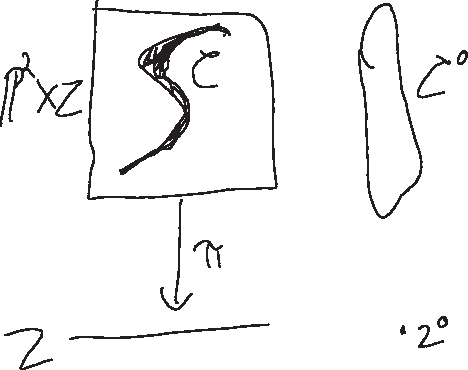
\includegraphics[width=0.5\textwidth]{2011-02-09_Diagram_001}\end{center}
        
        The \emph{fiber} $\mathcal C^0 = \pi^{-1}(z^0)$ of $\mathcal C$ over a point $z^0\in Z$ is the curve whose equation is the polynomial obtained.
        
        by substituting $z_\nu^0$ for $z_\nu$.  The 3 partial derivatives $F_x$, $F_y$, $F_z$ are polynomials in $x$, $y$, $z$, $\{z_\nu\}$ linear in $z_\nu$ and homogeneous of degree $d - 1$ in $x$, $y$, $z$.  They define some subvariety of $\mathbb P^2\times Z$.  Let $S$ be the variety $\{F_1 = F_2 = F_3 = 0\}$.  Note that $S \subset \mathcal C$ (by Euler).
        
        The fiber $\mathcal C^0$ over a point $z^0$ of $Z$ is smooth if and only if $\mathcal C^0$ doesn't meet $S$.
        
        We can construct $\Sigma = \pi(S)$ the image of $S$ via a polynomial $\mathbb P^2 \times Z \to Z$.  Later we'll prove that the image of the projection of any Zariski closed subvariety of $\mathbb P^2 \times Z$ to $Z$ is also Zariski closed.
        
        So the set $\Sigma$ is closed in the affine space $Z$.  But $\Sigma$ is not all of $Z$ (because the Fermat curve is smooth).  So $\Sigma \subset Z$ is a proper closed subvariety.  So the set of $z^0$ for which $\mathcal C^0$ is smooth is a Zariski open subset of $\mathbb A^N$.
      \end{proof}
\end{notessection}


\begin{notessection}{2}{11}{2011}
  Last time, we gave a proof that almost every plane curve of degree $d$ is smooth parameter space $\mathbb A^N$ : $N = \binom{d+2}{2}$.
  
  Another proof, continuing from the middle of the last one:
  \begin{proof}
    The dimension of $S$ (as defined last time) is $N + 2 - 3 = N - 1$ (the three from $F_x = F_y = F_z = 0$).  So $\pi(S)$ is at most $N - 1$ dimensional, and so it's $\overline{\pi(S)}$.  But $\dim Z = N$, so $\overline{\pi(S)} \ne Z$.
  \end{proof}
  
  \paragraph{Some words about topology} $\mathbb A^N= \mathbb C^N$ is a complex variety of dimension $N$. As a real manifold, it's dimension is $2N$.
  In the complex topology, you can have closed disks, e.g. $|z| \le 1$ (has positive measure).  In the Zariski topology, closed subsets have no measure.  e.g., in $\mathbb C$, the only closed subsets are finite point sets.  In $\mathbb C^2$, $V(ax + by + c)$ has no measure (it's a complex plane (dimension 1)).
  
  \begin{prop*}
    A smooth curve $C$ of degree 3 in $\mathbb P^2$ contains exactly 9 flex points.
  \end{prop*}
  \begin{proof}
    Let $f$ be a cubic defining $C$.  The second partial derivatives of $f$ are linear, so the determinant of the Hessian is a cubic polynomial which defines the Hessian curve $H$.
    \begin{thm*}[B\'ezout's theorem]
      A curve of degree $m$ in $\mathbb{P}^2$ intersects a curve of degree $n$ in exactly $mn$ points.
    \end{thm*}
    By this theorem (not yet proved), the two cubics $C$ and $H$ intersect in 9 points.  One can show that the multiplicities are one, and that $C$ and $H$ don't have a factor in common.  Thus, we get exactly 9 flexes.
  \end{proof}
  
  \begin{eg*}
    $y^2 = x^3 - x$ \\
    homogenization gives $y^2z = x^3 - xz^2$ \\
    Then \fbox{$f = x^3 - xz^2 - y^2z$}. \\
    The Hessian matrix is $$\begin{bmatrix} 6x & 0 & -2z \\ 0 & -2z & -2y \\ -2z & -2y & -2x \end{bmatrix}$$
    Then $H(f) = 8(3zx^2 - 3y^2x + z^3)$.  \\
    The flexes: You can eliminate $z$ from $f = H(f) = 0$.  Then you get a homogeneous polynomial in $x$ and $y$.  You can solve for $x / y$, let $y$ be 1, and then plug back in and solve for $z$.  In this example, we get that one of the flex points is at $(x:y:z) = (0:1:0)$.
  \end{eg*}
  
  \subsection*{Genus and Euler characteristic}
    Goal: Want to understand the topological structure of smooth plane curves.
    
    It's useful to put them in a family.  Notation as above.  Let $U = Z  - \Sigma = Z - \pi(S)$.  This is the parameter space for smooth plane curves of degree $d$.  The smooth plane curves are the fibers of the projection $\mathcal C\subset \mathbb P^2 \times U$ to $U$.  
    
    \begin{prop*}
      All the smooth curves of degree $d$ are homeomorphic to each other (as real manifolds of dimension 2).
    \end{prop*}
    \begin{proof}
      The problem set shows that $U$ is path-connected (in the complex topology).  Connect the two points in $U$ (which correspond to curves in $\mathbb P^2 \times U$) by a path.
      
      \begin{center}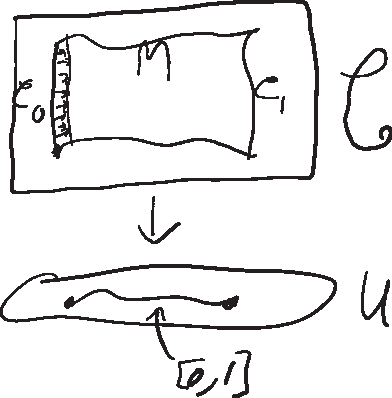
\includegraphics[width=0.5\textwidth]{2011-02-11_Diagram_001}\end{center}
      
      We have a function $f: M \to [0, 1]$.  Define a diffeomorphism by taking the gradient of $f$, and look at the gradient flow.  This tells us how to identify the fibers.
    \end{proof}
    
    \begin{cor*}
      Smooth plane curves are orientable, connected surfaces.
    \end{cor*}
    \begin{proof}
      Orientability is simple.  To orient a smooth surface, we must give a continuously varying orientation to the tangent planes.  But tangent plane is a $\mathbb C$-vector space (of dimension one, $\sum f_i(p) v_i = U$).  So multiplying any tangent vector by $i$ defines a counterclockwise rotation by $90^\circ$, which orients the tangent plane.
      
      We'll do connected next time.
    \end{proof}
  
\end{notessection}


\begin{notessection}{2}{14}{2011}
  
\end{notessection}


\begin{notessection}{2}{16}{2011}
  \subsection{Plane curves}
    monomials $m_1, \ldots, m_N$, coefficients $z_1,\ldots, z_N$
    \begin{align*}
      Z & = \text{the space of all homogeneous polynomials of degree $d$ in $x$, $y$, and $z$} \\
        & = \text{affine space with coordinates $z_\nu$}
    \end{align*}
    (We have $f(x, y, z) = z_1x^d + z_2 x^{d-1} + \cdots$)
    
    $U = $ open subset in $Z$ corresponding to smooth plane curves
    
    $\mathcal C \subset \mathbb P^2 \times Z$
    
    $$
    \xymatrix{
    \mathcal C \ar[drr] & \subset & \mathbb P^2 \times Z \ar[d] && \mathcal C|_U = \mathcal C_U \ar[drr] & \subset & \mathbb P^2 \times U \ar[d] \\
                       &         &  Z                           && && U
    }
    $$
    
    \begin{prop*}
      Smooth plane curves are orientable and connected surfaces, and compact.
    \end{prop*}
    \begin{proof}
      Oreintability was done last time.
      
      To check connectedness, we just need to check one smooth curve of degree $d$ is connected.  $\mathcal C : \{ x^d + y^d - z^d = 0 \}$.
      
      Look at the line $y = z$.  On $U_2$, taking $z = 1$ we have $x^d + y^d = 1$.  Since $y = z$, $y = 1$, and then $x^d = 0$.  Since this is a root of order $d$, $C$ meets this line in only one point.  This means that it's connected. (WHY?)
    \end{proof}
    
    Given a connected, orientable, compact surface, it's topologically characterized by $g = \text{the genus} = \text{the \# of holes}$.
    
    \begin{defn*}
      The \emph{Euler characteristic} of $C$ is $2 - 2g$.
    \end{defn*}
    
    The Euler characteristic can be computed used an arbitrary triangulation, and then $E = \text{\# vertices} - \text{\# edges} + \text{\# faces}$.
    
    A sphere is, topologically, a tetrahedron, we have that the Euler characteristic is $4 - 6 + 4 = 2$.  We can do a similar thing for a torus.
    
    What is the Euler characteristic and genus of a smooth plane curve of degree $d$?
    
    Let's represent a smooth plane curve as a branched cover of $\mathbb P^1$.
    
    \begin{enumerate}[{Method }I]
      \item Start with the Fermat curve, and do an explicit calculation.  $C: \{x^d + y^d - z^d = 0\}$ \\
        Taking $z = 1$, $U_2 \simeq \mathbb A^2 \simeq \mathbb C^2$.  Then we have $x^d + y^d = 1$.  Drop $y$ by projection.
        Fix a value $x_0$ for $x$.  Then the line $y = x_0$ intersects the curve in $\le d$ points.
        Typically, we get $d$ values for $y$.
        \begin{enumerate}[{Case }I]
          \item $x_0^d \ne 1$.  Solve $y^d = 1 - x_0^d$.  There are $d$ solution s (if $y$ is a solution, then so is $yr^{2 \pi i j / d}$ for $0 \le j \le d$)
          \item $x_0^d = 1$.  Solve $y^d = 0$.  The only solution is $y = 0$. Now we look at $x_0$.  Triangulate $\mathbb P^1$, which is a sphere, as follows.  There are $d$ values for $x_0$, $x_i^d = 1$, $x_i = e^{2\pi i j / d}$.  
      \begin{center}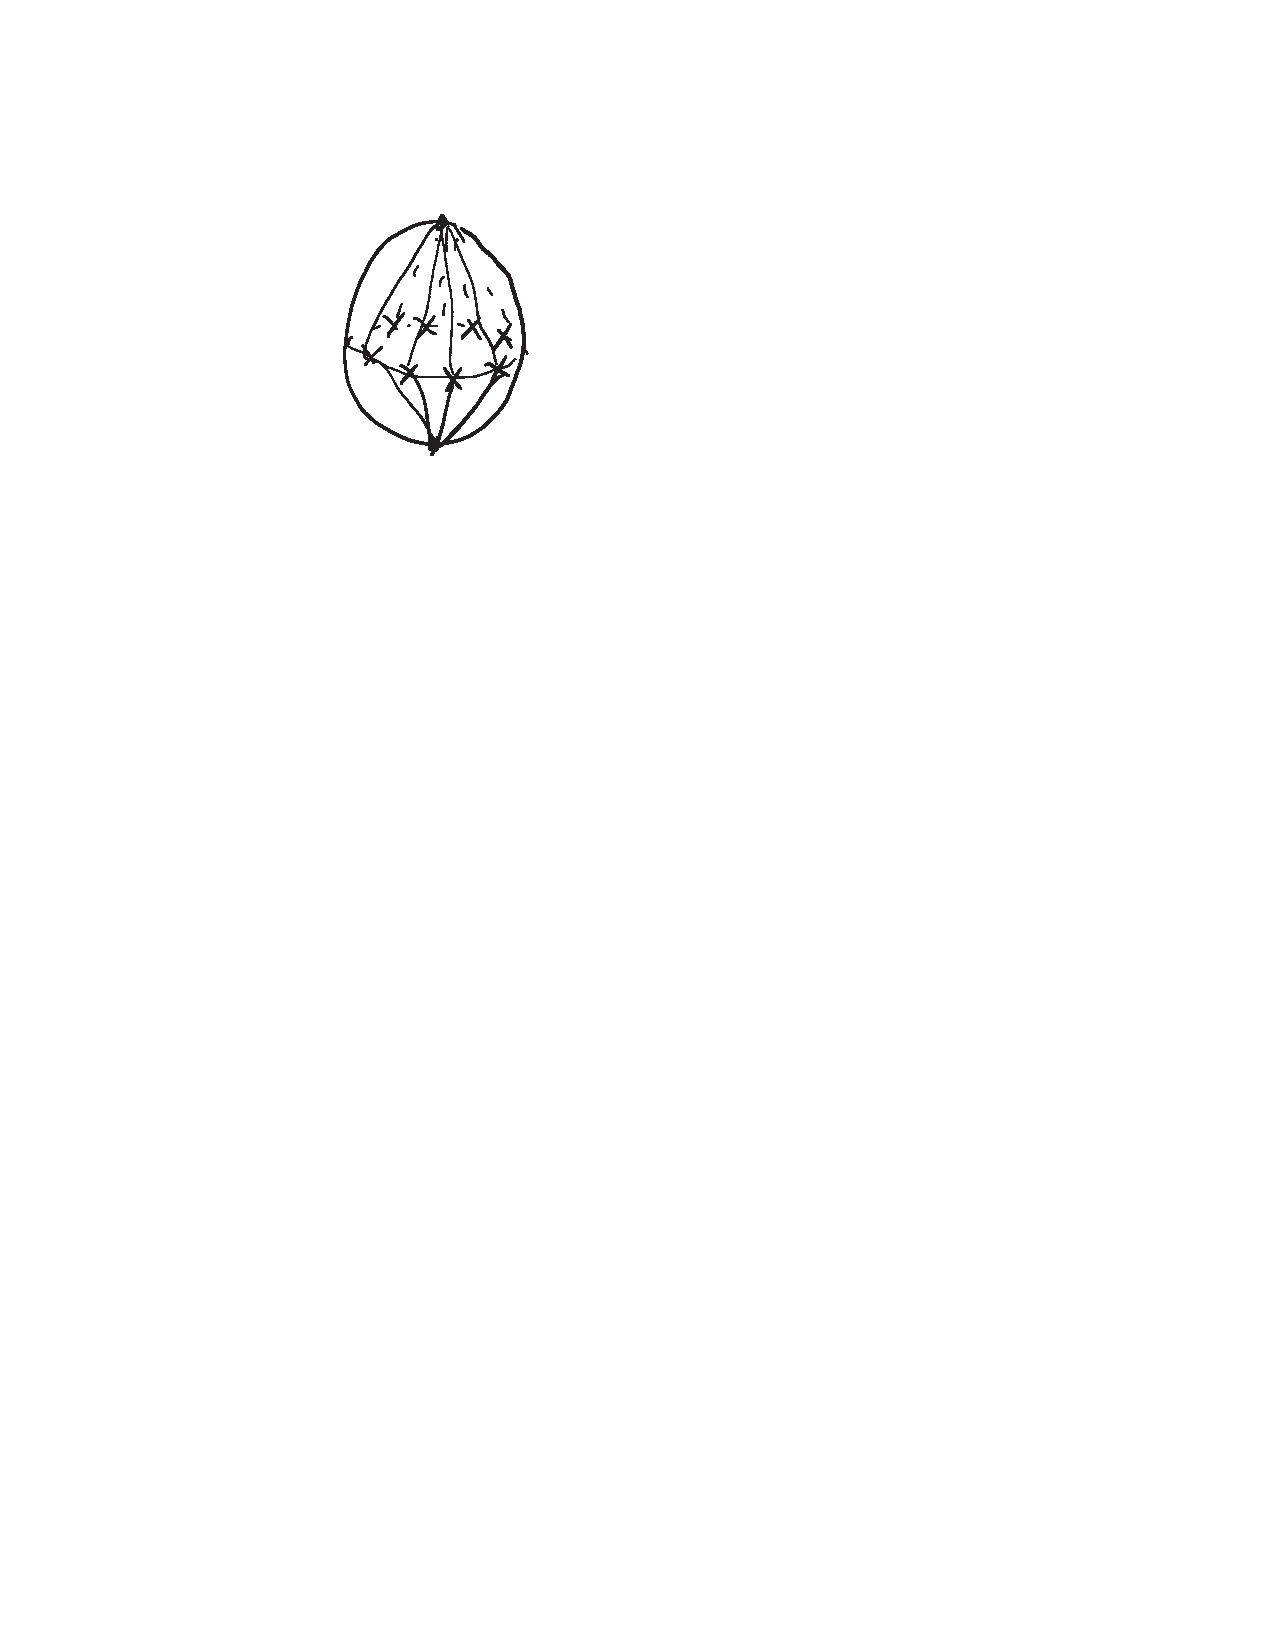
\includegraphics[width=0.5\textwidth]{2011-02-14_Diagram_001}\end{center}
          These points distribute themselves along the equator of $\mathbb P^1$.  Adding points at the poles, there are $2 + d$ vertices, $d + d + d = 3d$ edges, and $2d$ faces, which gives us 2. This is what happens ``downstairs'' (in the projected curve onto $X = \mathbb P^1$).\\
          Upstairs, there is an induced triangulation:
          \begin{itemize}
            \item vertices: $d + d + d = 3d$
            \item edges: $3d^2$
            \item faces: $2d^2$
          \end{itemize}
          Then the Euler characteristic is $E = 3d- 3d^2 + 2d^2 = 3d - d^2 = d(3 - d)$.  Then $g = \frac12(d - 1)(d - 2)$.
        \end{enumerate}
      \item Let $C$ be a smooth curve of degree $d$.  Assume the coefficient of $z^d$ is not zero.  Divide by that coefficient, giving $f(x, y, z) = z^d - a_1(x, y) z^{d-1} + \cdots \pm a_d(x, y)$.  Homogenous polynomial $\implies$ $a_i(x, y)$ is degree $i$ in $x$ and $y$.  Then drop $z$ by projection onto $\mathbb P^1(x, y)$.
        
        Fix $(x_0, y_0)$.  View $z^d - a_1(x_0, y_0) z^{d-1} + \cdots \pm a_d(x_0, y_0) = 0$ as a polynomial of degree $d$ in $z$.  Typically this has $d$ roots, but for some values of $(x, y)$, there are $d-1$ roots.
        
        There is a polynomial $\Delta$, discriminant, degree $d(d - 1)$ in $x$ and $y$.  $\Delta = 0$ iff there are less than $d$ roots.  (The discriminant for a quadratic is $b^2 - 4ac$.  It tells you whether or not the polynomial has double roots.)  (Note, if the discriminant has only simple roots, then the claim above (that there are only $d$ or $d - 1$ roots at any point) is intuitively/geometrically true.)
        
        Triangulate $X = \mathbb P^1$ by putting vertices at these $d(d - 1)$ points.  For $\mathbb P^1$, the Euler characteristic is $2$.  Pulling the triangulation up, the Euler characteristic is approximately $2d$ (everything gets multiplied by $d$).  However, we placed the vertices at the $d(d - 2)$ points where there are $d - 1$ roots.  Then the Euler characteristic is $2d - d(d - 1) = 3d - d^2$.
    \end{enumerate}
\end{notessection}

\end{document}